\documentclass{extbook}[14pt]
\usepackage{multicol, enumerate, enumitem, hyperref, color, soul, setspace, parskip, fancyhdr, amssymb, amsthm, amsmath, bbm, latexsym, units, mathtools}
\everymath{\displaystyle}
\usepackage[headsep=0.5cm,headheight=0cm, left=1 in,right= 1 in,top= 1 in,bottom= 1 in]{geometry}
\usepackage{dashrule}  % Package to use the command below to create lines between items
\newcommand{\litem}[1]{\item #1

\rule{\textwidth}{0.4pt}}
\pagestyle{fancy}
\lhead{}
\chead{Answer Key for Progress Quiz 10 Version A}
\rhead{}
\lfoot{6232-9639}
\cfoot{}
\rfoot{Fall 2020}
\begin{document}
\textbf{This key should allow you to understand why you choose the option you did (beyond just getting a question right or wrong). \href{https://xronos.clas.ufl.edu/mac1105spring2020/courseDescriptionAndMisc/Exams/LearningFromResults}{More instructions on how to use this key can be found here}.}

\textbf{If you have a suggestion to make the keys better, \href{https://forms.gle/CZkbZmPbC9XALEE88}{please fill out the short survey here}.}

\textit{Note: This key is auto-generated and may contain issues and/or errors. The keys are reviewed after each exam to ensure grading is done accurately. If there are issues (like duplicate options), they are noted in the offline gradebook. The keys are a work-in-progress to give students as many resources to improve as possible.}

\rule{\textwidth}{0.4pt}

\begin{enumerate}\litem{
Describe the end behavior of the polynomial below.
\[ f(x) = -8(x - 4)^{4}(x + 4)^{5}(x + 9)^{3}(x - 9)^{4} \]

The solution is the graph below, which is option B.
\begin{center}
    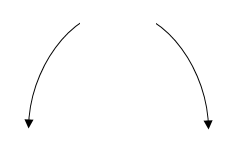
\includegraphics[width=0.3\textwidth]{../Figures/polyEndBehaviorBA.png}
\end{center}\begin{enumerate}[label=\Alph*.]
\begin{multicols}{2}
\item 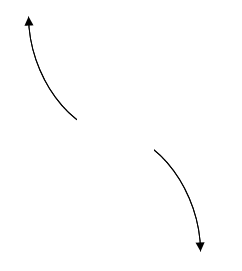
\includegraphics[width = 0.3\textwidth]{../Figures/polyEndBehaviorAA.png}
\item 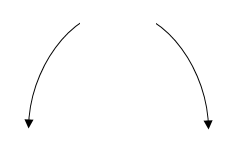
\includegraphics[width = 0.3\textwidth]{../Figures/polyEndBehaviorBA.png}
\item 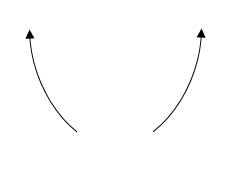
\includegraphics[width = 0.3\textwidth]{../Figures/polyEndBehaviorCA.png}
\item 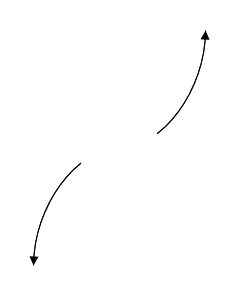
\includegraphics[width = 0.3\textwidth]{../Figures/polyEndBehaviorDA.png}
\end{multicols}\item None of the above.\end{enumerate}
\textbf{General Comment:} Remember that end behavior is determined by the leading coefficient AND whether the \textbf{sum} of the multiplicities is positive or negative.
}
\litem{
Construct the lowest-degree polynomial given the zeros below. Then, choose the intervals that contain the coefficients of the polynomial in the form $x^3+bx^2+cx+d$.
\[ -3 - 4 i \text{ and } 3 \]

The solution is \( x^{3} +3 x^{2} +7 x -75 \), which is option D.\begin{enumerate}[label=\Alph*.]
\item \( b \in [-1.9, 1.65], c \in [0.21, 3.58], \text{ and } d \in [-17, -10] \)

$x^{3} + x^{2} +x -12$, which corresponds to multiplying out $(x + 4)(x -3)$.
\item \( b \in [-1.9, 1.65], c \in [-0.45, 0.03], \text{ and } d \in [-10, -4] \)

$x^{3} + x^{2} -9$, which corresponds to multiplying out $(x + 3)(x -3)$.
\item \( b \in [-3.44, -2.63], c \in [6.39, 7.85], \text{ and } d \in [73, 79] \)

$x^{3} -3 x^{2} +7 x + 75$, which corresponds to multiplying out $(x-(-3 - 4 i))(x-(-3 + 4 i))(x + 3)$.
\item \( b \in [2.57, 3.6], c \in [6.39, 7.85], \text{ and } d \in [-75, -74] \)

* $x^{3} +3 x^{2} +7 x -75$, which is the correct option.
\item \( \text{None of the above.} \)

This corresponds to making an unanticipated error or not understanding how to use nonreal complex numbers to create the lowest-degree polynomial. If you chose this and are not sure what you did wrong, please contact the coordinator for help.
\end{enumerate}

\textbf{General Comment:} Remember that the conjugate of $a+bi$ is $a-bi$. Since these zeros always come in pairs, we need to multiply out $(x-(-3 - 4 i))(x-(-3 + 4 i))(x-(3))$.
}
\litem{
Describe the zero behavior of the zero $x = -8$ of the polynomial below.
\[ f(x) = -9(x + 5)^{3}(x - 5)^{2}(x - 8)^{6}(x + 8)^{3} \]

The solution is the graph below, which is option D.
\begin{center}
    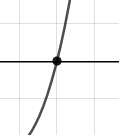
\includegraphics[width=0.3\textwidth]{../Figures/polyZeroBehaviorCopyDA.png}
\end{center}\begin{enumerate}[label=\Alph*.]
\begin{multicols}{2}
\item 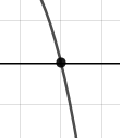
\includegraphics[width = 0.3\textwidth]{../Figures/polyZeroBehaviorCopyAA.png}
\item 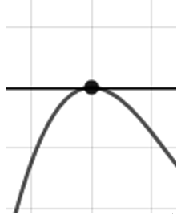
\includegraphics[width = 0.3\textwidth]{../Figures/polyZeroBehaviorCopyBA.png}
\item 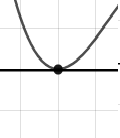
\includegraphics[width = 0.3\textwidth]{../Figures/polyZeroBehaviorCopyCA.png}
\item 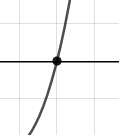
\includegraphics[width = 0.3\textwidth]{../Figures/polyZeroBehaviorCopyDA.png}
\end{multicols}\item None of the above.\end{enumerate}
\textbf{General Comment:} You will need to sketch the entire graph, then zoom in on the zero the question asks about.
}
\litem{
Construct the lowest-degree polynomial given the zeros below. Then, choose the intervals that contain the coefficients of the polynomial in the form $ax^3+bx^2+cx+d$.
\[ \frac{7}{5}, 5, \text{ and } \frac{3}{2} \]

The solution is \( 10x^{3} -79 x^{2} +166 x -105 \), which is option D.\begin{enumerate}[label=\Alph*.]
\item \( a \in [6, 13], b \in [-51, -48], c \in [-22, -13], \text{ and } d \in [97, 108] \)

$10x^{3} -51 x^{2} -16 x + 105$, which corresponds to multiplying out $(5x + 7)(x -5)(2x -3)$.
\item \( a \in [6, 13], b \in [43, 51], c \in [-30, -22], \text{ and } d \in [-111, -103] \)

$10x^{3} +49 x^{2} -26 x -105$, which corresponds to multiplying out $(5x + 7)(x + 5)(2x -3)$.
\item \( a \in [6, 13], b \in [-80, -75], c \in [161, 167], \text{ and } d \in [97, 108] \)

$10x^{3} -79 x^{2} +166 x + 105$, which corresponds to multiplying everything correctly except the constant term.
\item \( a \in [6, 13], b \in [-80, -75], c \in [161, 167], \text{ and } d \in [-111, -103] \)

* $10x^{3} -79 x^{2} +166 x -105$, which is the correct option.
\item \( a \in [6, 13], b \in [70, 80], c \in [161, 167], \text{ and } d \in [97, 108] \)

$10x^{3} +79 x^{2} +166 x + 105$, which corresponds to multiplying out $(5x + 7)(x + 5)(2x + 3)$.
\end{enumerate}

\textbf{General Comment:} To construct the lowest-degree polynomial, you want to multiply out $(5x -7)(x -5)(2x -3)$
}
\litem{
Which of the following equations \textit{could} be of the graph presented below?

\begin{center}
    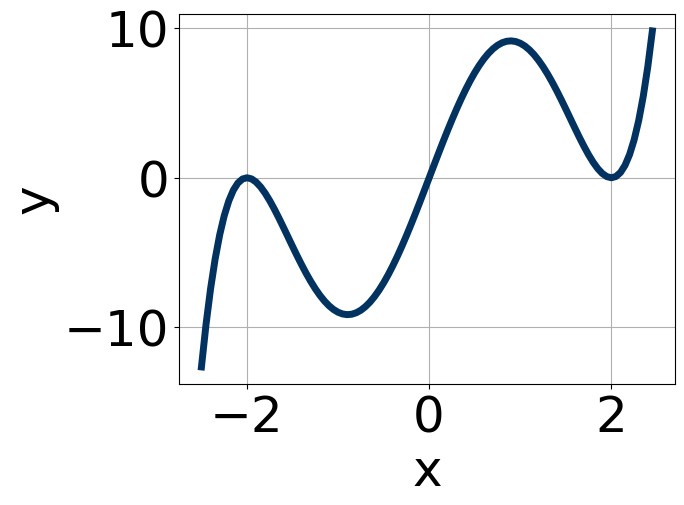
\includegraphics[width=0.5\textwidth]{../Figures/polyGraphToFunctionA.png}
\end{center}




The solution is \( 17x^{7} (x - 2)^{6} (x + 2)^{4} \), which is option B.\begin{enumerate}[label=\Alph*.]
\item \( 18x^{10} (x - 2)^{6} (x + 2)^{9} \)

The factor $(x + 2)$ should have an even power and the factor $x$ should have an odd power.
\item \( 17x^{7} (x - 2)^{6} (x + 2)^{4} \)

* This is the correct option.
\item \( -9x^{8} (x - 2)^{8} (x + 2)^{6} \)

The factor $x$ should have an odd power and the leading coefficient should be the opposite sign.
\item \( 16x^{7} (x - 2)^{8} (x + 2)^{7} \)

The factor $(x + 2)$ should have an even power.
\item \( -14x^{9} (x - 2)^{8} (x + 2)^{10} \)

This corresponds to the leading coefficient being the opposite value than it should be.
\end{enumerate}

\textbf{General Comment:} General Comments: Draw the x-axis to determine which zeros are touching (and so have even multiplicity) or cross (and have odd multiplicity).
}
\litem{
Describe the zero behavior of the zero $x = -3$ of the polynomial below.
\[ f(x) = 7(x - 3)^{9}(x + 3)^{10}(x - 8)^{6}(x + 8)^{7} \]

The solution is the graph below, which is option B.
\begin{center}
    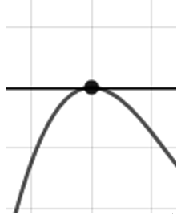
\includegraphics[width=0.3\textwidth]{../Figures/polyZeroBehaviorBA.png}
\end{center}\begin{enumerate}[label=\Alph*.]
\begin{multicols}{2}
\item 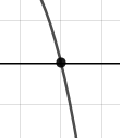
\includegraphics[width = 0.3\textwidth]{../Figures/polyZeroBehaviorAA.png}
\item 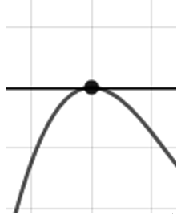
\includegraphics[width = 0.3\textwidth]{../Figures/polyZeroBehaviorBA.png}
\item 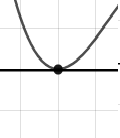
\includegraphics[width = 0.3\textwidth]{../Figures/polyZeroBehaviorCA.png}
\item 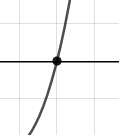
\includegraphics[width = 0.3\textwidth]{../Figures/polyZeroBehaviorDA.png}
\end{multicols}\item None of the above.\end{enumerate}
\textbf{General Comment:} You will need to sketch the entire graph, then zoom in on the zero the question asks about.
}
\litem{
Describe the end behavior of the polynomial below.
\[ f(x) = -9(x + 3)^{2}(x - 3)^{3}(x - 8)^{3}(x + 8)^{4} \]

The solution is the graph below, which is option B.
\begin{center}
    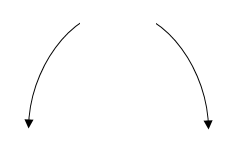
\includegraphics[width=0.3\textwidth]{../Figures/polyEndBehaviorCopyBA.png}
\end{center}\begin{enumerate}[label=\Alph*.]
\begin{multicols}{2}
\item 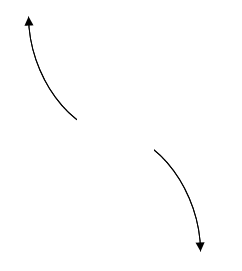
\includegraphics[width = 0.3\textwidth]{../Figures/polyEndBehaviorCopyAA.png}
\item 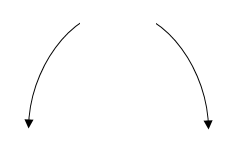
\includegraphics[width = 0.3\textwidth]{../Figures/polyEndBehaviorCopyBA.png}
\item 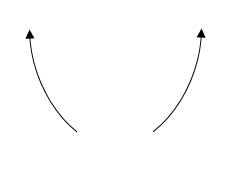
\includegraphics[width = 0.3\textwidth]{../Figures/polyEndBehaviorCopyCA.png}
\item 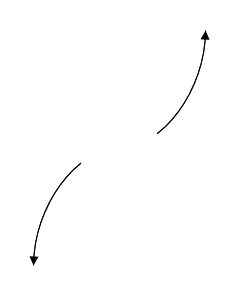
\includegraphics[width = 0.3\textwidth]{../Figures/polyEndBehaviorCopyDA.png}
\end{multicols}\item None of the above.\end{enumerate}
\textbf{General Comment:} Remember that end behavior is determined by the leading coefficient AND whether the \textbf{sum} of the multiplicities is positive or negative.
}
\litem{
Construct the lowest-degree polynomial given the zeros below. Then, choose the intervals that contain the coefficients of the polynomial in the form $x^3+bx^2+cx+d$.
\[ -2 - 5 i \text{ and } -1 \]

The solution is \( x^{3} +5 x^{2} +33 x + 29 \), which is option C.\begin{enumerate}[label=\Alph*.]
\item \( b \in [-6.2, -3.4], c \in [31, 34.2], \text{ and } d \in [-29.2, -25] \)

$x^{3} -5 x^{2} +33 x -29$, which corresponds to multiplying out $(x-(-2 - 5 i))(x-(-2 + 5 i))(x -1)$.
\item \( b \in [-3.3, 2.4], c \in [5.7, 6.4], \text{ and } d \in [2.1, 6.8] \)

$x^{3} + x^{2} +6 x + 5$, which corresponds to multiplying out $(x + 5)(x + 1)$.
\item \( b \in [1.6, 5.7], c \in [31, 34.2], \text{ and } d \in [27.5, 30.4] \)

* $x^{3} +5 x^{2} +33 x + 29$, which is the correct option.
\item \( b \in [-3.3, 2.4], c \in [-1.2, 4.8], \text{ and } d \in [0, 3.6] \)

$x^{3} + x^{2} +3 x + 2$, which corresponds to multiplying out $(x + 2)(x + 1)$.
\item \( \text{None of the above.} \)

This corresponds to making an unanticipated error or not understanding how to use nonreal complex numbers to create the lowest-degree polynomial. If you chose this and are not sure what you did wrong, please contact the coordinator for help.
\end{enumerate}

\textbf{General Comment:} Remember that the conjugate of $a+bi$ is $a-bi$. Since these zeros always come in pairs, we need to multiply out $(x-(-2 - 5 i))(x-(-2 + 5 i))(x-(-1))$.
}
\litem{
Which of the following equations \textit{could} be of the graph presented below?

\begin{center}
    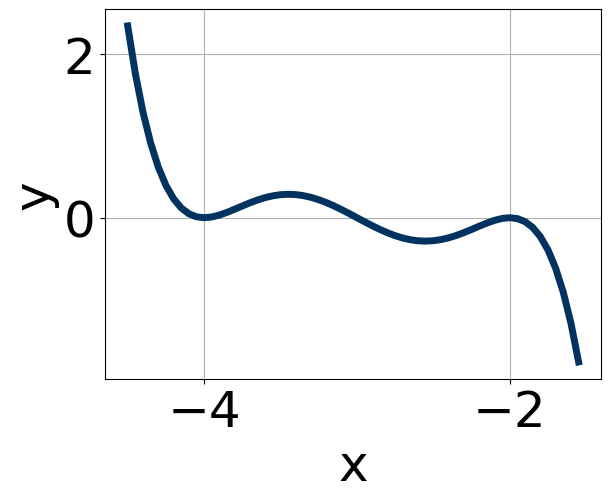
\includegraphics[width=0.5\textwidth]{../Figures/polyGraphToFunctionCopyA.png}
\end{center}




The solution is \( -9(x + 2)^{6} (x + 4)^{8} (x + 3)^{11} \), which is option D.\begin{enumerate}[label=\Alph*.]
\item \( -7(x + 2)^{4} (x + 4)^{7} (x + 3)^{10} \)

The factor $(x + 4)$ should have an even power and the factor $(x + 3)$ should have an odd power.
\item \( 2(x + 2)^{6} (x + 4)^{6} (x + 3)^{6} \)

The factor $(x + 3)$ should have an odd power and the leading coefficient should be the opposite sign.
\item \( 20(x + 2)^{6} (x + 4)^{6} (x + 3)^{7} \)

This corresponds to the leading coefficient being the opposite value than it should be.
\item \( -9(x + 2)^{6} (x + 4)^{8} (x + 3)^{11} \)

* This is the correct option.
\item \( -15(x + 2)^{8} (x + 4)^{5} (x + 3)^{5} \)

The factor $(x + 4)$ should have an even power.
\end{enumerate}

\textbf{General Comment:} General Comments: Draw the x-axis to determine which zeros are touching (and so have even multiplicity) or cross (and have odd multiplicity).
}
\litem{
Construct the lowest-degree polynomial given the zeros below. Then, choose the intervals that contain the coefficients of the polynomial in the form $ax^3+bx^2+cx+d$.
\[ \frac{7}{5}, \frac{-3}{4}, \text{ and } \frac{5}{3} \]

The solution is \( 60x^{3} -139 x^{2} +2 x + 105 \), which is option A.\begin{enumerate}[label=\Alph*.]
\item \( a \in [60, 69], b \in [-143, -136], c \in [2, 9], \text{ and } d \in [100, 106] \)

* $60x^{3} -139 x^{2} +2 x + 105$, which is the correct option.
\item \( a \in [60, 69], b \in [-69, -57], c \in [-129, -122], \text{ and } d \in [100, 106] \)

$60x^{3} -61 x^{2} -128 x + 105$, which corresponds to multiplying out $(5x + 7)(4x -3)(3x -5)$.
\item \( a \in [60, 69], b \in [-143, -136], c \in [2, 9], \text{ and } d \in [-109, -102] \)

$60x^{3} -139 x^{2} +2 x -105$, which corresponds to multiplying everything correctly except the constant term.
\item \( a \in [60, 69], b \in [24, 32], c \in [-153, -147], \text{ and } d \in [-109, -102] \)

$60x^{3} +29 x^{2} -152 x -105$, which corresponds to multiplying out $(5x + 7)(4x + 3)(3x -5)$.
\item \( a \in [60, 69], b \in [138, 144], c \in [2, 9], \text{ and } d \in [-109, -102] \)

$60x^{3} +139 x^{2} +2 x -105$, which corresponds to multiplying out $(5x + 7)(4x -3)(3x + 5)$.
\end{enumerate}

\textbf{General Comment:} To construct the lowest-degree polynomial, you want to multiply out $(5x -7)(4x + 3)(3x -5)$
}
\end{enumerate}

\end{document}